\documentclass[a4paper]{article}
\usepackage[a4paper, total={7in, 9in}]{geometry}
\usepackage{ctex} % 引入ctex包处理中文  
\usepackage{fancyhdr} % 引入fancyhdr包来定制页眉和页脚  
\usepackage{refcount} % 引入refcount包来获取标签的页码  
\usepackage{lastpage}
\usepackage{ulem} % 导入 ulem 包
\usepackage{listings}
\usepackage{xcolor}
\usepackage{graphicx}
\usepackage{float}
\usepackage{tabularx}
\usepackage{array}

\lstset{
    language=Python,
    basicstyle=\ttfamily\footnotesize,
    keywordstyle=\color{blue},
    commentstyle=\color{green},
    stringstyle=\color{red},
    numbers=left,
    numberstyle=\tiny\color{gray},
    stepnumber=1,
    numbersep=10pt,
    backgroundcolor=\color{lightgray},
    frame=single,
    breaklines=true,
    captionpos=b,
    showspaces=false,
    showstringspaces=false,
    showtabs=false,
    tabsize=4
}

\pagestyle{plain} % 这是默认的页面样式,通常不显示页眉和页脚  
\fancypagestyle{mainmatter}{
	\fancyhf{} % 清除默认的页眉和页脚设置
	\lhead{Team \# 2024062828349}
	\rhead{Page \thepage{} of \pageref{LastPage}} % 显示当前页码和最后一页的页码 
	\fancyfoot[C]{\thepage}
}
\begin{document}
	% 设置3号黑体并居中
	\begin{center}
		\fontsize{16pt}{19pt}\selectfont \textbf{2024年第三届“钉钉杯”大学生}  

		\fontsize{16pt}{19pt}\selectfont
		\textbf{大数据挑战赛论文}
		
		% 题目  
		\centering
		题目:
		\textbf{\underline{基于ARIMAX、LSTM与集成学习框架的烟草产品销售预测研究}}
		
	\end{center}
	\pagenumbering{gobble}
	% 摘要和关键字环境
	\begin{abstract}
		\fontsize{12pt}{15pt}\selectfont
		\textbf{烟草产业}作为我国经济体系中的一支关键支柱,鉴于其独特的属性以及国家实施的专营体制,对其进行销售预测显得尤为重要,以辅助政策制定及商业策略规划。本项研究聚焦于某特定区域内多品牌烟草商品的销售数据分析,目标在于\textbf{预测未来的销售量与销售额},从而为决策层提供有力的数据支持。所分析的数据集涵盖了五个特定品牌,即A1、A2、A3、A4与A5,这些品牌的月度销售历史记录。
		
		针对首个研究问题,本研究采用\textbf{ARIMAX(自回归积分滑动平均模型与外生变量)}和\textbf{LSTM(长短期记忆网络)}对A1与A2两个品牌的销售量进行深入分析及预测。通过将历史销售数据与相关的外部变量相结合,并进行\textbf{模型参数}的优化调整,我们得以获取对未来销售量的预测值。
		
		对于第二个研究议题,A3与A4品牌的销售额预测,则运用了\textbf{ARIMA(自回归积分滑动平均模型)与Prophet}两种模型。ARIMA模型通过\textbf{差分处理与参数微调},有效管理时间序列数据;而Prophet模型则通过\textbf{分解趋势、季节性变化及节假日}影响,实现了销售额的精准预测。
		
		第三个研究方向致力于\textbf{提升预测精度与稳健性},为此,我们构建了一个集成学习框架,对A5品牌的销售量与销售额进行综合预测。该集成学习模型整合了\textbf{ARIMA、Prophet、XGBoost以及LSTM}等多种模型,借助多模型融合的优势,充分发挥各自在预测领域的长处,最终实现了更为准确的预测结果。
		
		就模型性能评估而言,我们采用了诸如\textbf{准确率(Accuracy)、F1-Score、AUC}等一系列指标进行综合考量。实证分析显示,\textbf{集成学习}模型在预测A5品牌销售量与销售额时,展现出了较高的准确度与可靠性。
		
		综上所述,本研究不仅证实了时间序列预测模型在烟草销售预测领域的适用性,同时也彰显了集成学习策略在增强预测效能方面的潜在价值。这一发现为烟草行业提供了宝贵的见解,\textbf{有助于其销售策略的制定与市场预测的优化}。

		\vspace{3\baselineskip}

		\textbf{关键词:时间序列预测\hspace{0.5cm}ARIMA模型\hspace{0.5cm}集成学习\hspace{0.5cm}烟草销售数据\hspace{0.5cm}预测准确性}


	\end{abstract}  
	\newpage  
	
	% 目录
	\tableofcontents  
	\newpage 
	
	\pagestyle{mainmatter}
	\pagenumbering{arabic}
	\setcounter{page}{1}
	\section{问题重述}
	\subsection{问题背景}
	

	\subsection{数据分析}

	
	\subsubsection{销量预测}

	
	\textbf{数据预处理}
	

	\textbf{模型建立}
	
	
	\textbf{预测结果}
	

	\textbf{数据预处理}

	
	\textbf{模型建立}
	
	
	\textbf{预测结果}
	
	
	\subsubsection{联合预测}
	
	
	\textbf{模型建立}
	
	
	\textbf{预测结果}
	
	
	\subsection{问题提出}
	\textbf{(1)问题一:对未来销量进行预测}:
	\textbf{(2)问题二:对销售金额进行预测}:
	\textbf{(3)问题三:集成学习}:
	\section{问题分析}
	\subsection{问题1分析}
		\begin{figure}[H]
			\centering
			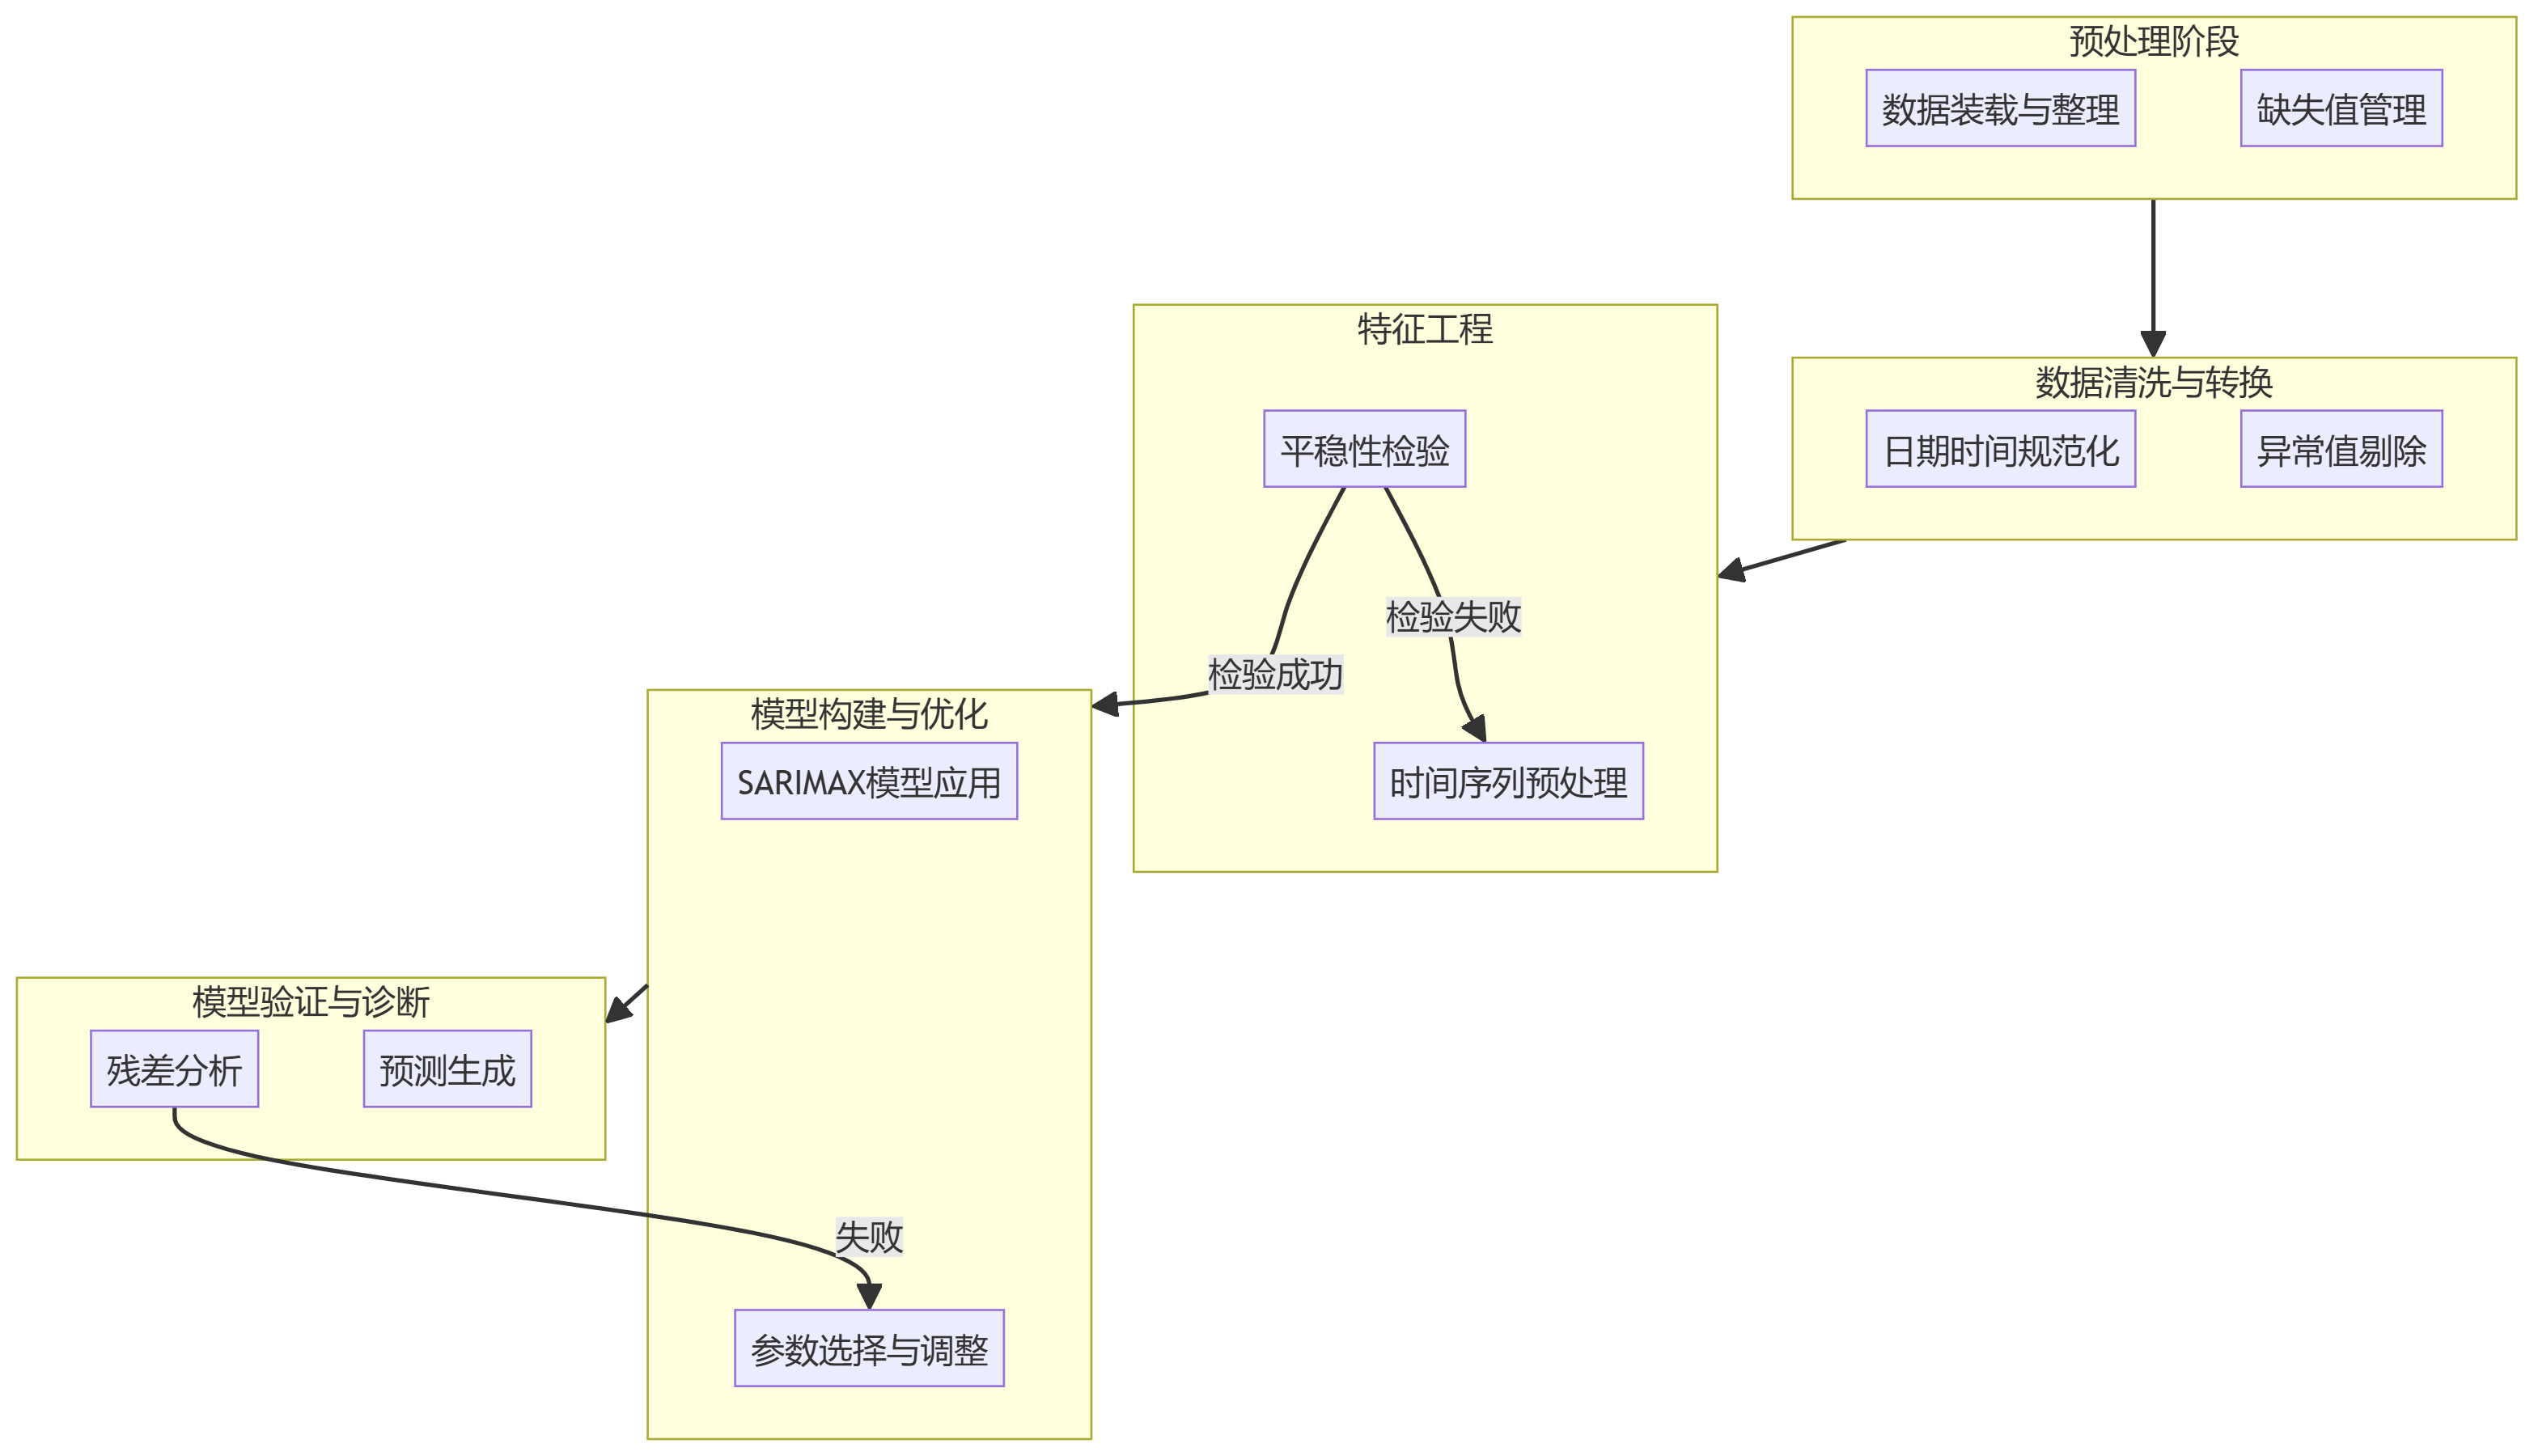
\includegraphics[width=1.0\textwidth]{img/Q1_analysis.png}
		\end{figure}

		\subsection{问题2分析}
		\begin{figure}[H]
		\centering
		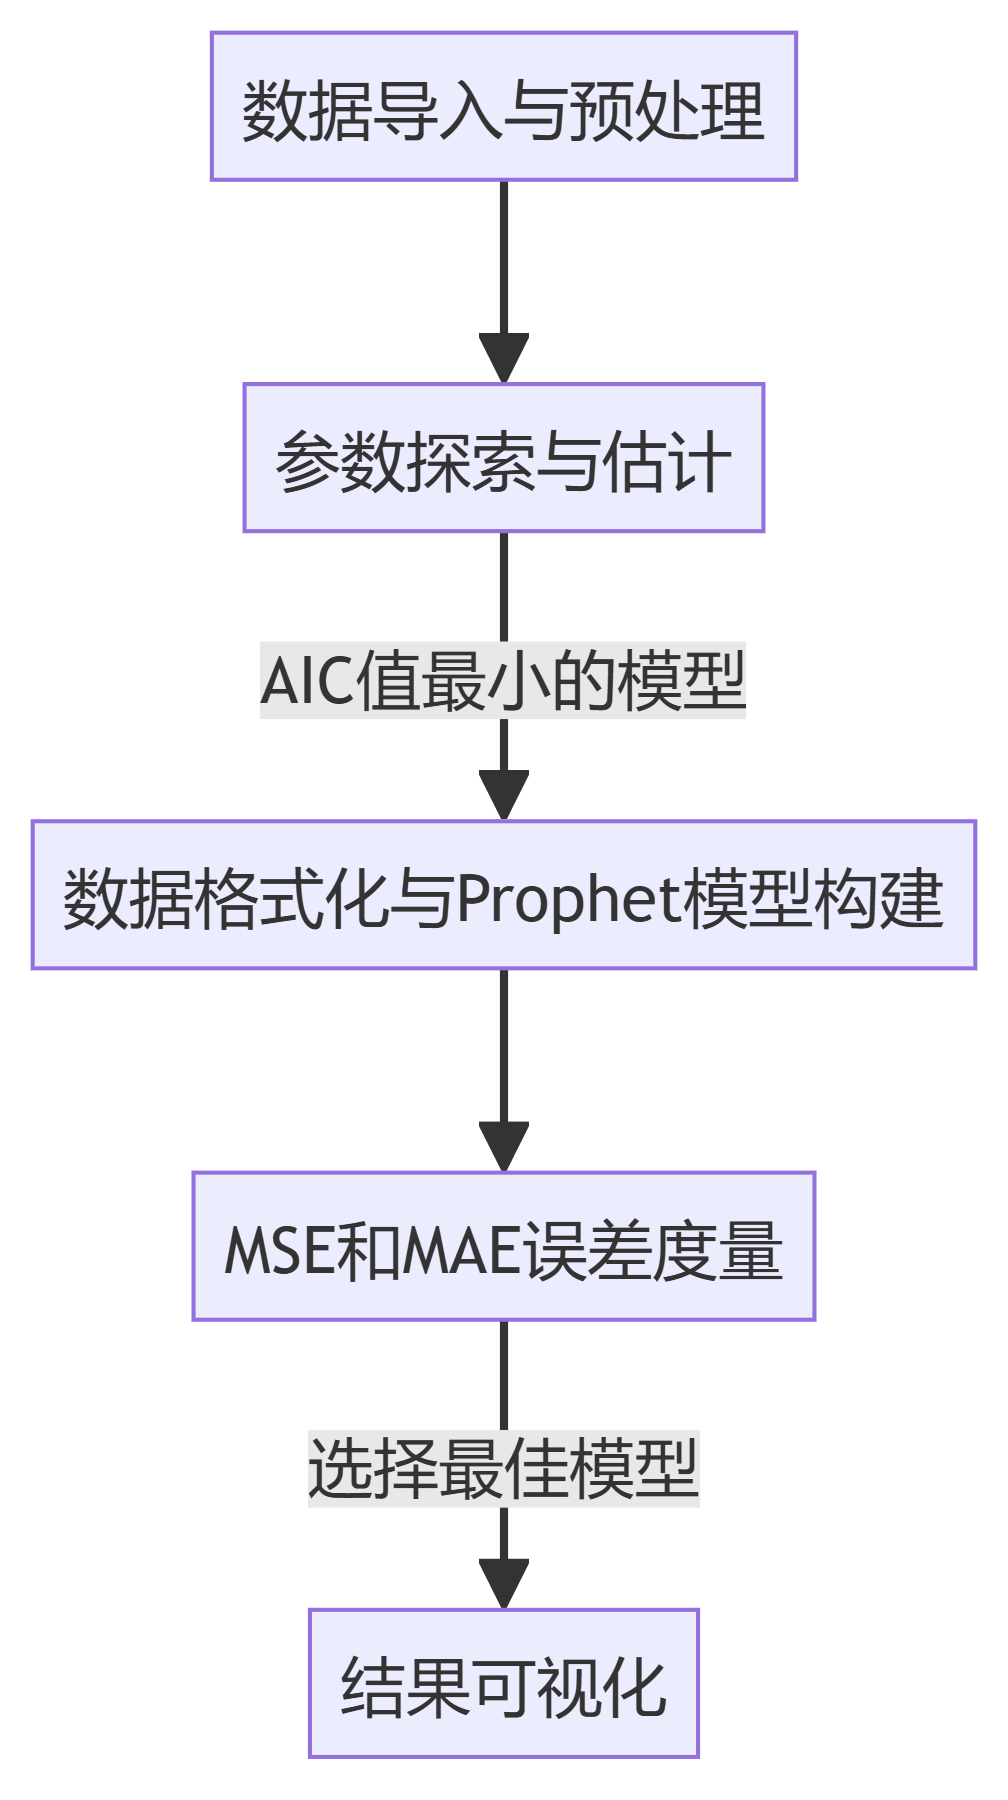
\includegraphics[width=0.3\textwidth]{img/Q2_analysis.png}
	\end{figure}
	\subsection{问题3分析}
	

	\section{模型假设}
	
	\begin{enumerate}


	\end{enumerate}

	\section{模型的建立与求解}  
	\subsection{问题1的模型建立与求解}


	\begin{lstlisting}[caption={Python}, label={lst:example}]

	\end{lstlisting}

	在预测阶段,我们使用训练好的模型对未来的销量进行了预测。通过 $get\_forecast()$ 方法,我们获得了预测结果,并创建了一个新的时间索引来表示未来的时间段。将预测结果转换为一个 pd.Series 对象,并设置正确的时间索引,以确保预测数据的时间序列连续性。最终,我们绘制了历史数据和预测数据的时间序列图,以便于可视化对比,蓝色线表示历史数据,红色线表示预测结果。
	\begin{lstlisting}[caption={Python}, label={lst:example}]


	\end{lstlisting}


	\begin{figure}[H]
		\centering
		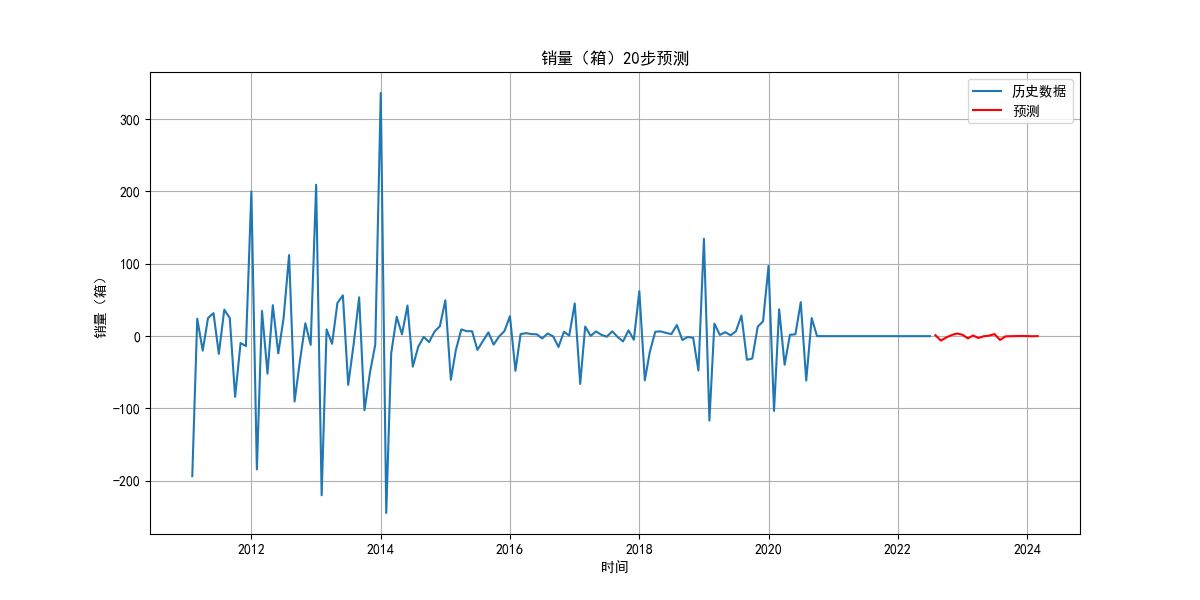
\includegraphics[width=1.0\textwidth]{img/A1_2.png}
	\end{figure}



	\setlength{\extrarowheight}{4pt}
	\begin{table}[H]

		\centering
	
		\begin{tabularx}{\textwidth}{|X|X|} % \textwidth是表格的总宽度
	
		\hline
	
		月份 & 预测销量(箱)\\
	
		\hline
	
		\hline
		2022-04-01 00:00:00	&73.46496951\\
		\hline
		2022-05-01 00:00:00	&74.12360938\\
	
		\hline
	
		\end{tabularx}
	
		\caption{表格}
	
	\end{table}


	\begin{figure}[H]
		\centering
		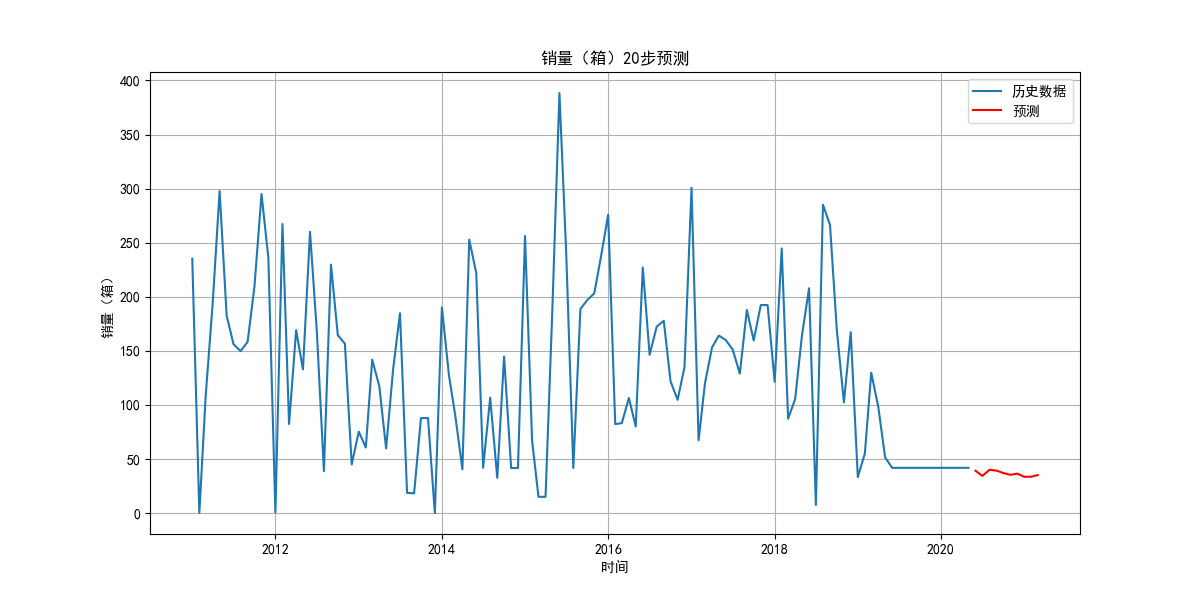
\includegraphics[width=1.0\textwidth]{img/A2_2.png}
	\end{figure}


	\setlength{\extrarowheight}{4pt}
	\begin{table}[H]
		\centering
		\begin{tabularx}{\textwidth}{|X|X|} % \textwidth是表格的总宽度
			\hline
			月份 & 预测销量(箱)\\
			\hline
			2020-04-01 00:00:00	&88.7035647\\
			\hline
		\end{tabularx}
	\end{table}
	\subsection{问题2的模型建立与求解}


	\textbf{绘制预测结果}


	\begin{figure}[H]
		\centering
		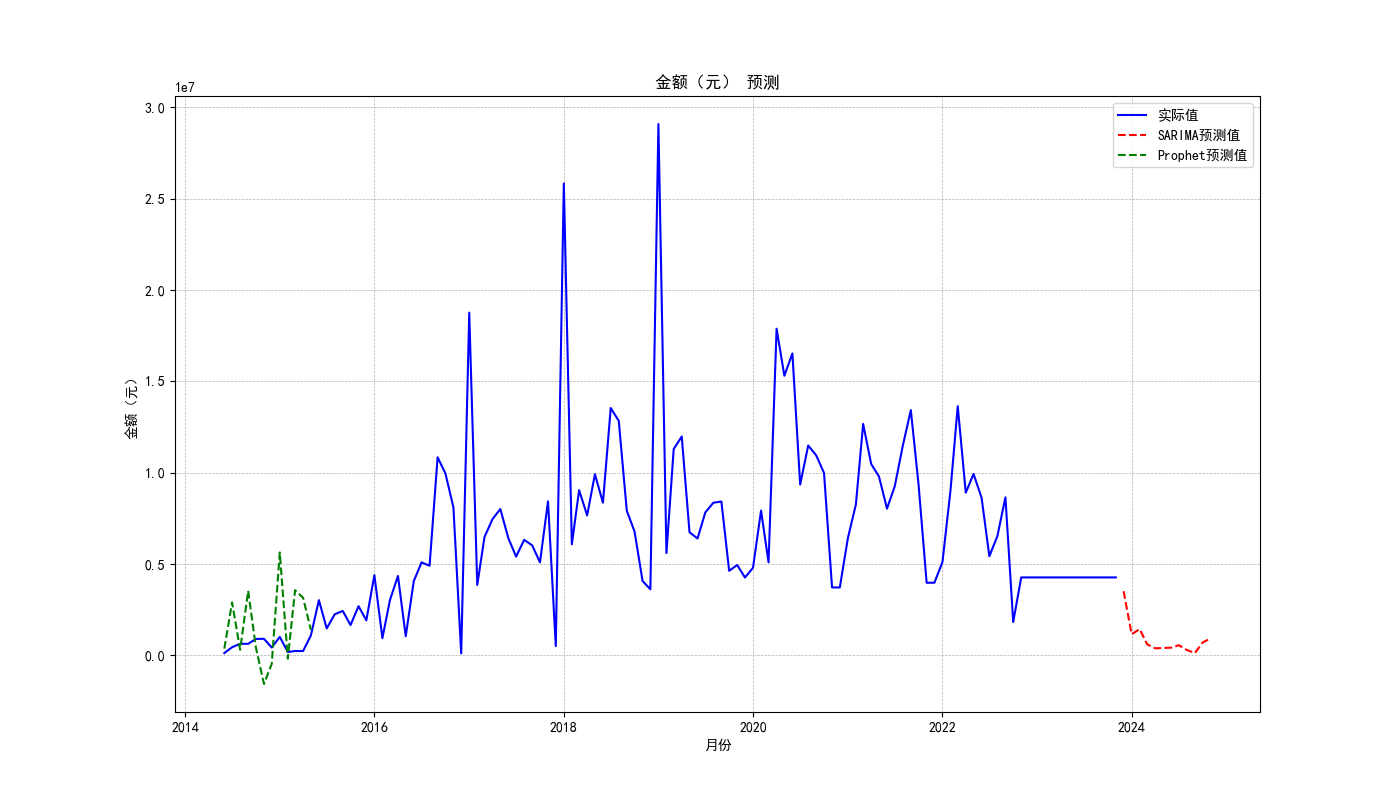
\includegraphics[width=0.9\textwidth]{img/Second_1.png}
		\caption{A3预测结果}
	\end{figure}
	\begin{figure}[H]
		\centering
		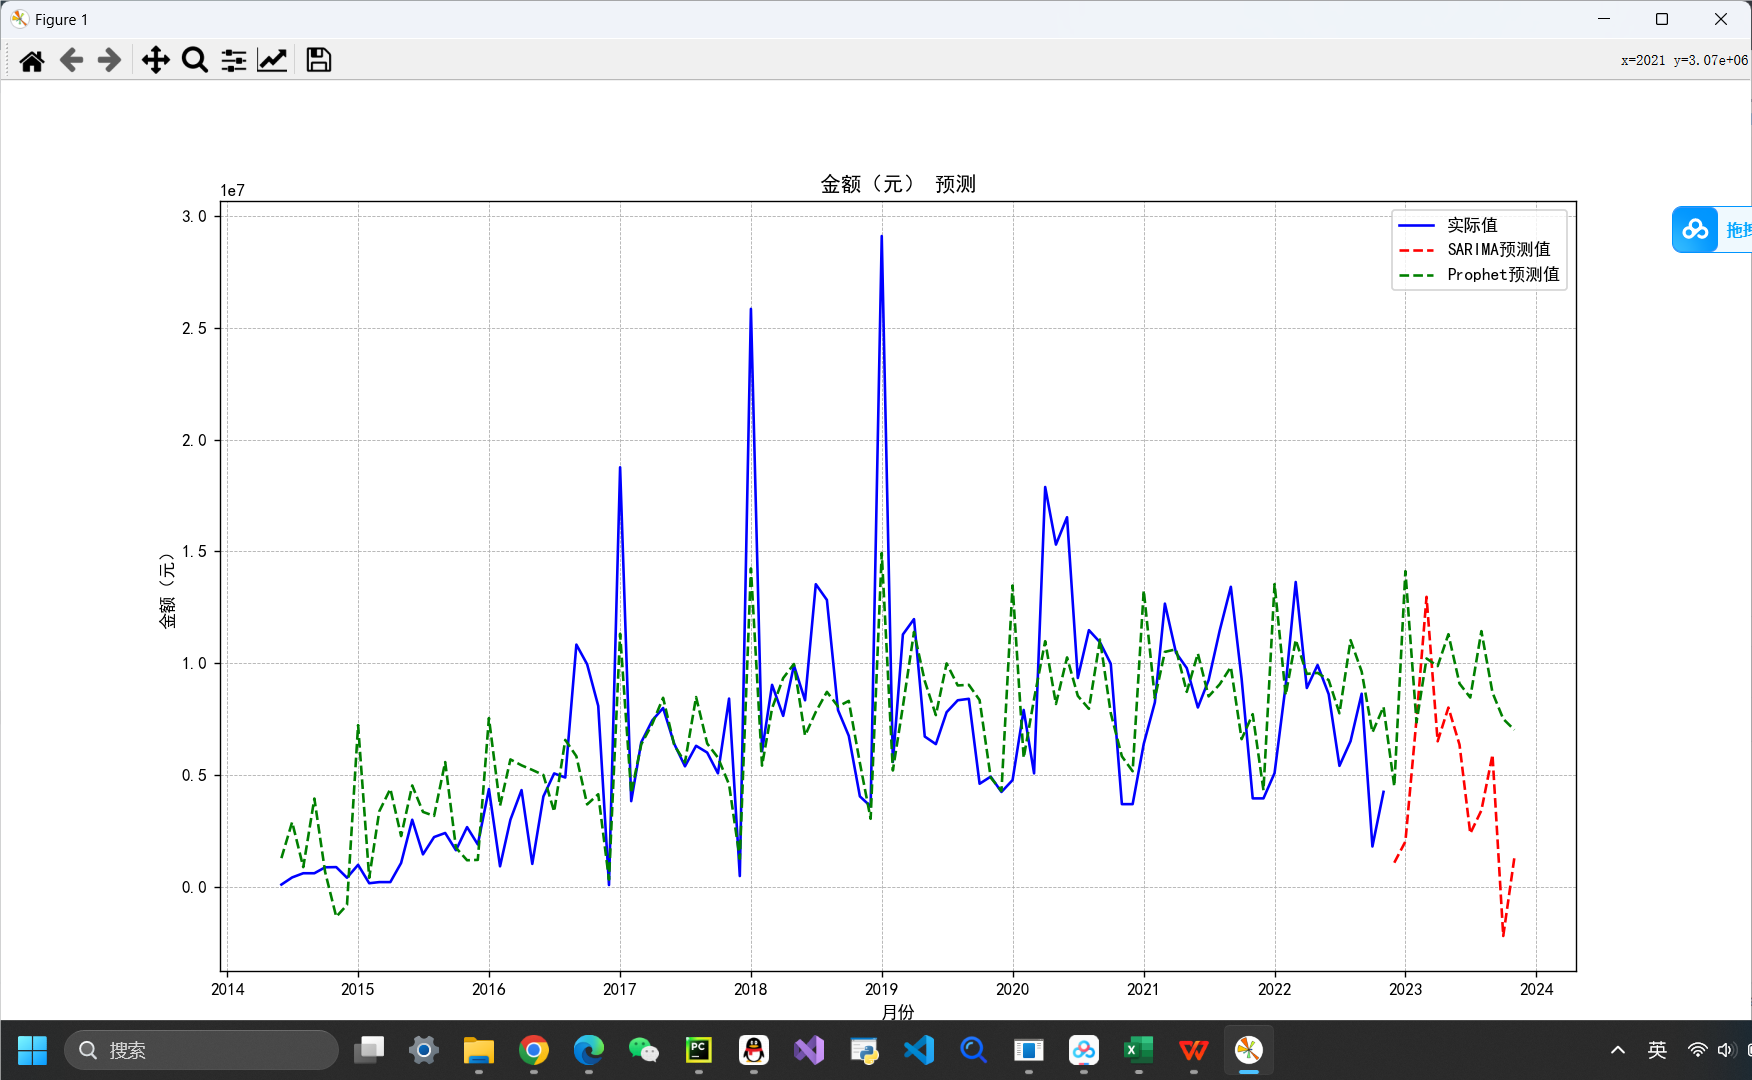
\includegraphics[width=0.9\textwidth]{img/Second_2.png}
		\caption{A4预测结果}
	\end{figure}

	\subsection{问题3的模型建立与求解}
	对于第三题,我们的任务是使用ARIMA、Prophet、XGBoost、LSTM四种模型对A5品牌的未来销量和销售金额进行预测,并通过集成学习模型(Stacking)来提升预测精度。这个任务涉及到时间序列预测和集成学习方法的应用。
	\subsubsection{数据预处理}
	为了确保模型可以正常训练和预测,首先需要对数据进行预处理,包括将月份转换为日期格式,设置索引,处理缺失值等步骤。

	\subsubsection{模型选择及训练}



	\begin{figure}[H]
		\centering
		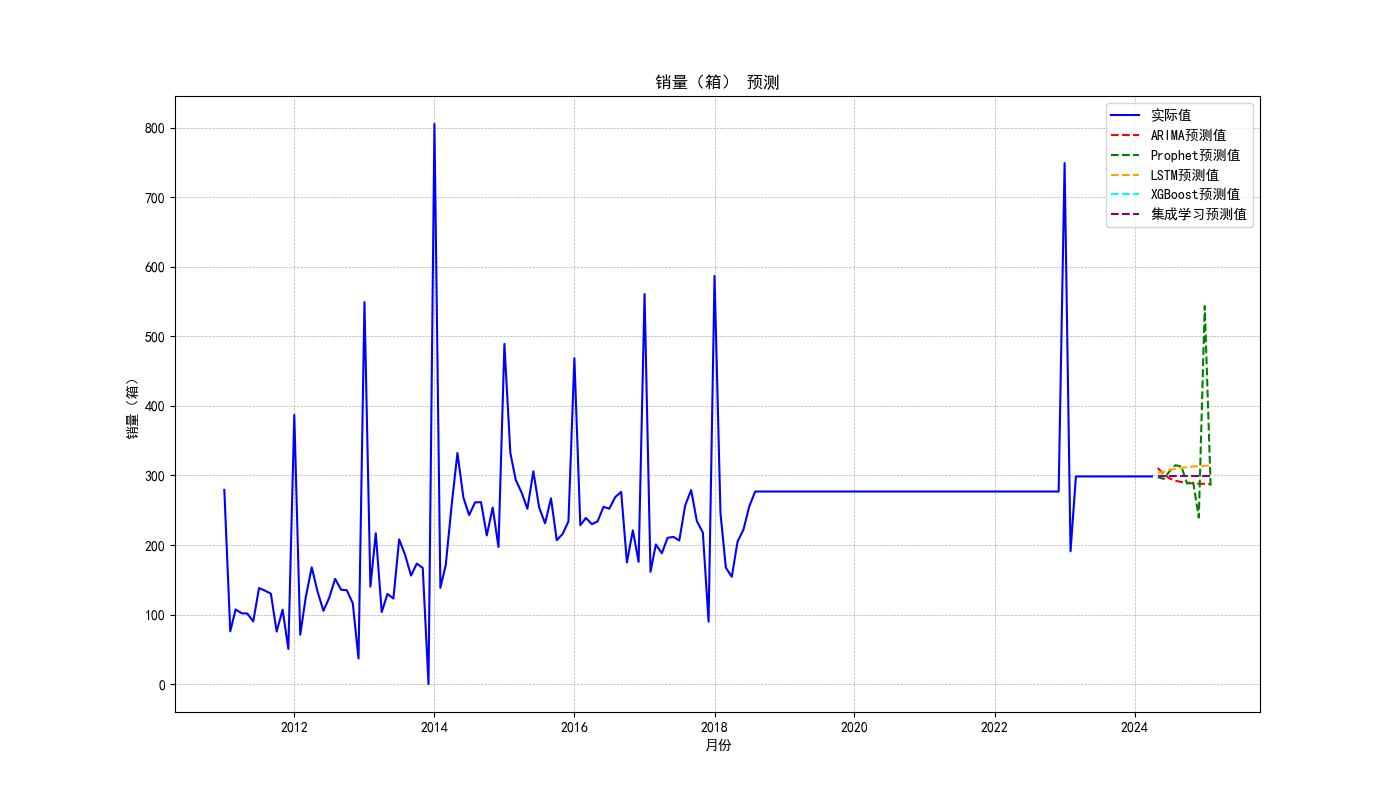
\includegraphics[width=1.0\textwidth]{img/3_1.png}
		\caption{销量预测结果}
	\end{figure}
	\begin{figure}[H]
		\centering
		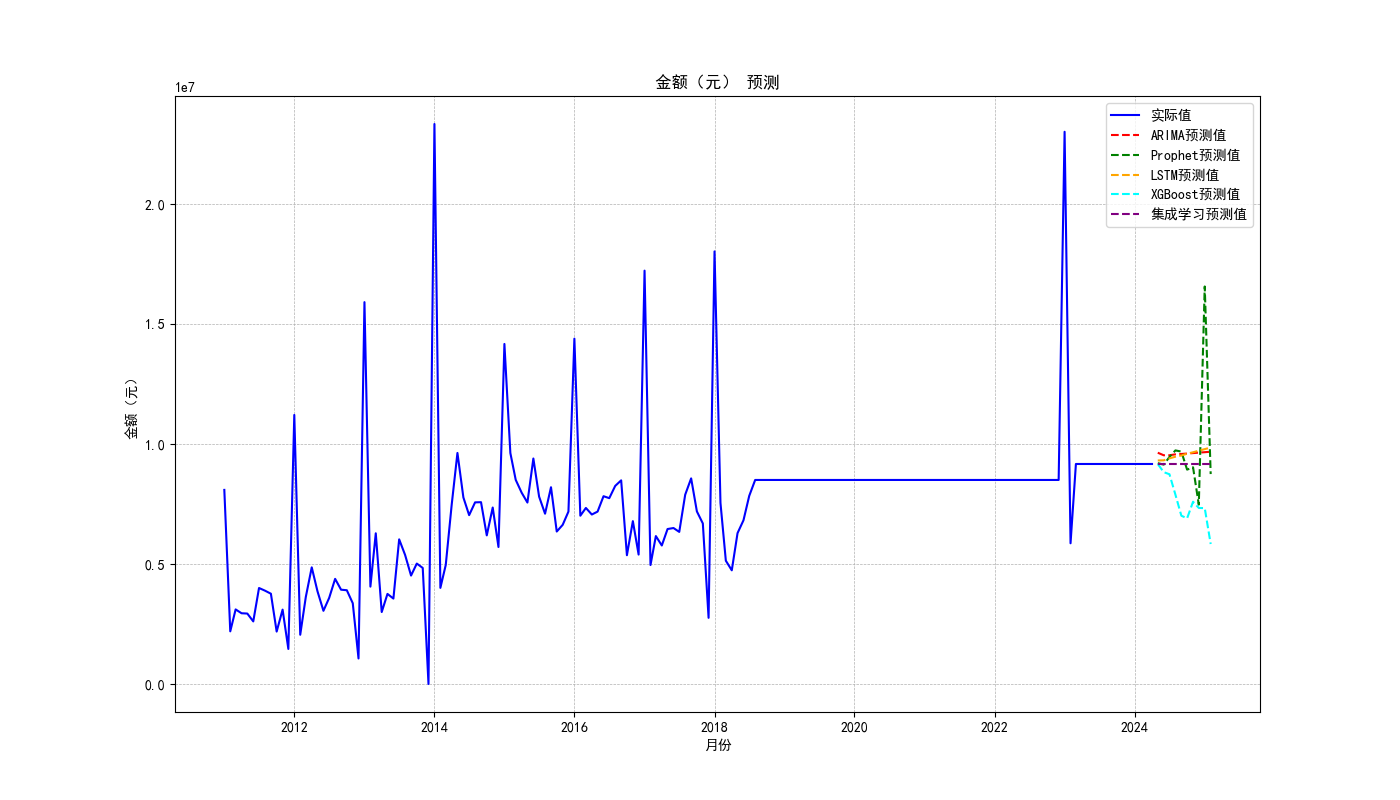
\includegraphics[width=1.0\textwidth]{img/3_2.png}
		\caption{金额预测结果}
	\end{figure}


	
	\section{模型的评价及优化}
	\subsection{误差分析}
	\subsection{模型的优点}
	\newpage
	\pagestyle{plain}
	\section{参考文献}
	\begin{thebibliography}{9}
		\bibitem{arima}
		程幸福 \hspace{2pt}陈厚铭 \hspace{2pt}樊红.季节ARIMA模型在企业销售量预测中的应用——以卷烟销售为例[A].中国商论.23.23 (2016): 167-168.
		\bibitem{pmdarima}
		谷秀娟 \hspace{2pt}梁润平.基才ARIMA模型的郑州市商品住宅销售价格预测研究[A].《金融理论与实践》.2012年第1期51-54
		\bibitem{pmdarima}
		刘璟瑶 \hspace{2pt}蒋辰宇 \hspace{2pt}陶杰.长短期记忆网络对销售量预测精度的影响[A].《财会研究》.2023年第6期76-80
		\bibitem{pmdarima}
		李融.基于XGBoost算法的跨境电商备货预测研究[A].《太原城市职业技术学院学报》.2024年第1期29-31,共3页
		\bibitem{pmdarima}
		杜红兵 \hspace{2pt}邢梦柯 \hspace{2pt}赵德超.Prophet-LSTM组合模型在运输航空征候预测中的应用[A].《安全与环境学报》.2024年第5期1878-1885,共8页
	\end{thebibliography}
	\newpage % 新的一页开始

	\section{附录}
	问题一代码:

	问题二代码:

	问题三代码:	
	
	
\end{document}